\documentclass[12pt,a4paper]{article} \usepackage[utf8]{inputenc} \usepackage[T1]{fontenc} \usepackage[brazil]{babel} \usepackage{geometry} \geometry{a4paper, margin=2.5cm} \usepackage{graphicx} \usepackage{hyperref} \usepackage{float} \title{Lab02 - IDP(Redes)} \author{Samuel Abrão 24101216} \date{\today} \begin{document} \maketitle \section*{Objetivos} Compreender o funcionamento de \textit{ping} e \textit{traceroute}, capturar e analisar pacotes ICMP/UDP no Wireshark, diferenciar ICMP de UDP no contexto dos comandos e interpretar os resultados coletados. \section*{Ping} O \textit{ping} testa conectividade fim a fim usando ICMP: envia \textit{Echo Request} e aguarda \textit{Echo Reply}. Na captura, os endereços IPv6 identificados nos pacotes ICMP foram, no papel de origem, \texttt{2804:14c:65a7:88b6:9b77:2\ldots} e, no papel de destino, \texttt{2800:3f0:4004:812::\ldots}; a Figura~\ref{fig:ipv6} mostra esses campos como vistos no Wireshark. Já os endereços IPv4 correspondentes estão evidenciados na Figura~\ref{fig:ipv4}, que apresenta a tela com os campos de origem/destino em IPv4 capturados. Em relação à quantidade de pacotes ICMP enviados e recebidos, o número exibido pelo Wireshark está sintetizado na Figura~\ref{fig:pacotes}. Sobre o TTL, recorde que é um contador de saltos para evitar loops; no \textit{ping} observamos o valor padrão utilizado no experimento como \textbf{113}, conforme evidência na Figura~\ref{fig:ttl}. Por fim, o RTT quantifica o tempo ida-e-volta de cada eco; as estatísticas do comando indicaram, com base na sua imagem, \textbf{min = 39{,}056 ms}, \textbf{avg = 39{,}929 ms}, \textbf{max = 40{,}802 ms} e \textbf{mdev = 0{,}873 ms}, conforme Figura~\ref{fig:rtt}. \begin{figure}[H] \centering 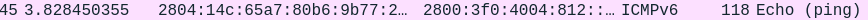
\includegraphics[width=\textwidth]{assets/ipv6.png} \caption{Ping: campos de origem/destino em IPv6 na captura.} \label{fig:ipv6} \end{figure} \begin{figure}[H] \centering 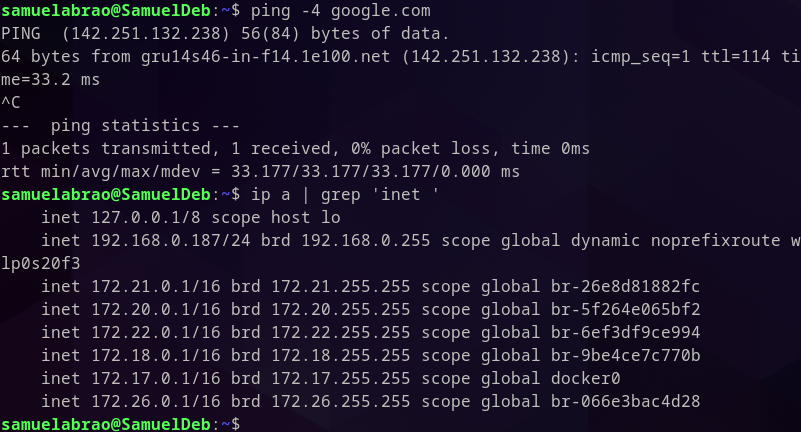
\includegraphics[width=\textwidth]{assets/ipv4.png} \caption{Ping: campos de origem/destino em IPv4 na captura.} \label{fig:ipv4} \end{figure} \begin{figure}[H] \centering 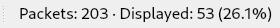
\includegraphics[width=\textwidth]{assets/pacotes.png} \caption{Resumo no Wireshark: quantidade de pacotes ICMP enviados/recebidos.} \label{fig:pacotes} \end{figure} \begin{figure}[H] \centering 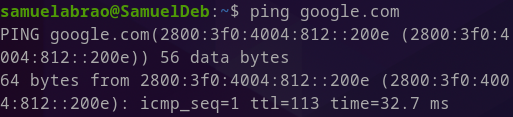
\includegraphics[width=\textwidth]{assets/ttl.png} \caption{TTL observado no experimento com \textit{ping} (valor padrão utilizado: 113).} \label{fig:ttl} \end{figure} \begin{figure}[H] \centering 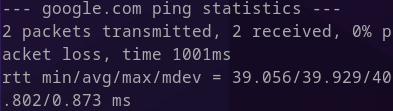
\includegraphics[width=\textwidth]{assets/rtt.png} \caption{Estatísticas de RTT do \textit{ping}: min/avg/max/mdev.} \label{fig:rtt} \end{figure} \section*{Traceroute} O \textit{traceroute} mapeia o caminho até o destino incrementando o TTL dos pacotes emitidos (1, 2, 3, \ldots); quando um roteador esgota o TTL, devolve ICMP \emph{Time Exceeded}, revelando-se como próximo salto. Na sua execução, a saída indica que o pacote não alcançou o destino \texttt{142.251.132.238}; o último salto com resposta válida foi o \textbf{14}, no roteador \texttt{216.239.54.237}, e, a partir daí, apareceram asteriscos. Assim, os saltos que responderam compõem o caminho parcial observado: \texttt{192.168.0.1} (\_gateway), \texttt{10.43.192.1}, \texttt{189.6.1.217} (\texttt{bd0601d9.virtua.com.br}), \texttt{189.6.2.168} (\texttt{bd0602a8.virtua.com.br}), endereços da operadora como \texttt{189.52.88.49}, \texttt{200.252.88.1}, \texttt{189.52.233.165}, seguido por \texttt{200.244.212.217} (\texttt{ebt-Plag-63-core02.bsasn.embratel.net.br}), \texttt{200.244.216.150} e \texttt{200.244.216.15} (core da Embratel em RJ), \texttt{200.244.19.96} e \texttt{201.39.52.58} (\texttt{peer-B54-agg03.rjo.embratel.net.br}), além de nós Google que responderam em tentativas alternadas como \texttt{216.239.42.152}, \texttt{142.251.240.190}, \texttt{209.85.240.106}, \texttt{216.239.54.237} e \texttt{209.85.240.94}. Em termos de TTL dos \textit{pacotes enviados}, o \textit{traceroute} parte de 1 e incrementa de 1 em 1 a cada tentativa; no Linux, o TTL padrão de emissão para tráfego IP geral é 64, mas, no \textit{traceroute}, o valor inicial é explicitamente controlado para provocar a resposta salto a salto. A Figura~\ref{fig:traceroute} ilustra a execução realizada. \begin{figure}[H] \centering 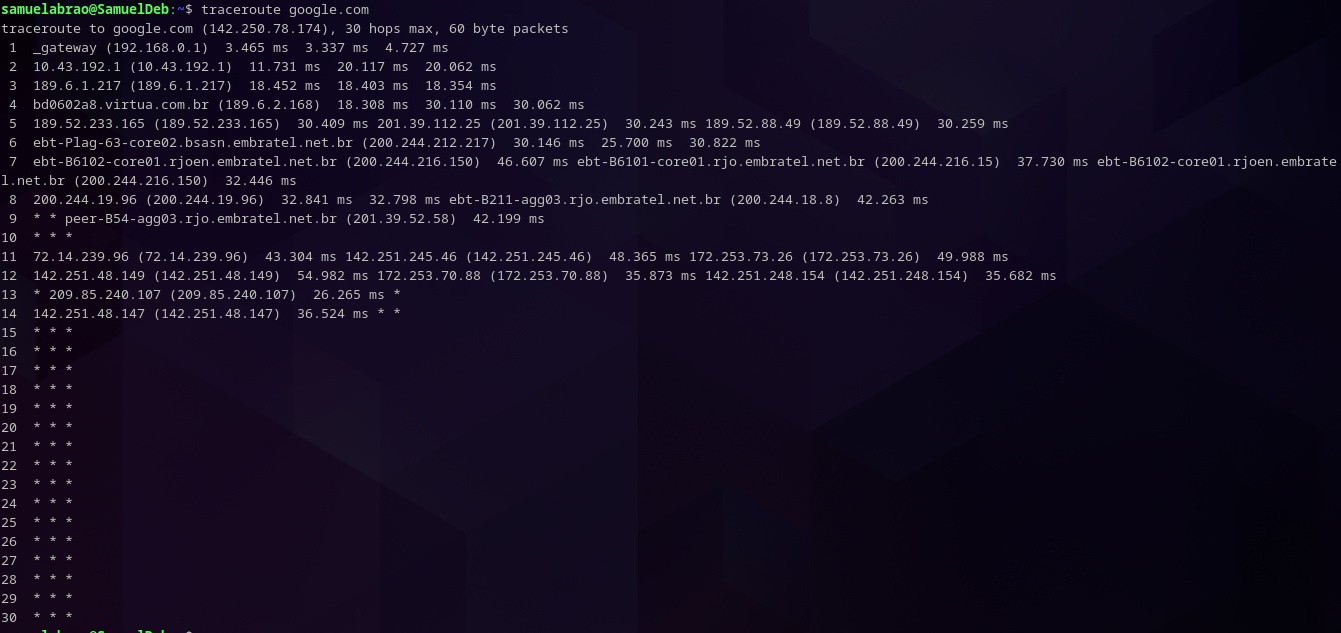
\includegraphics[width=\textwidth]{assets/traceroute.png} \caption{Execução do \textit{traceroute}: caminho até o salto 14, com interrupções posteriores.} \label{fig:traceroute} \end{figure} \end{document}